\section{Experiment 5: Point Cloud Experiment}
\label{sec:weberslaw}

%We conduct an additional experiment testing whether Weber's law applies to convolutional neural networks for graphical perception. For this, we generate three 2D point clouds as base stimuli -- each is created randomly by activating 10, 100, or 1000 pixels in a $100\times100$ raster image. We then additionally activate from 1 to 10 random pixels within the initial distribution but by carefully only selecting inactive pixels. We show examples for this in Fig.~\ref{fig:weber_law} (left). This means that the number of additional points is harder to identify if they are added to the 1000 pixel set while the 10 pixel set allows to easily count. We then let our networks solve a regression task to estimate the number of added points.

We also create a random 2D point cloud version of Weber's law, in which the networks must estimate the number of added dots (up to 10) over an initial number of 10, 100, or 1,000 dots (Fig.~\ref{fig:weber_law}). Each individual stimulus image has random dot placement. For 10 initial dots, \change{given a brief glance at the stimuli, a human can approximately estimate the number of the dots,} but for 100 and 1,000 initial dots, this is a difficult problem where a human is likely to randomly guess. For a CNN, this problem is also difficult: there are $\binom{100\times100}{10}=2.73\times10^{33}$ locations for the 10 initial dots, which makes memorization untenable.

%\subsection{Hypothesis}

\begin{hypolist}
	\item \textbf{H5.1} \textbf{The networks will be unable to solve the point cloud experiment.} This just-noticeable-difference problem has too many parameter variations to judge, though a human could solve the simplest version with 10 initial dots.
\end{hypolist}


\begin{figure}[tb]
  \centering
  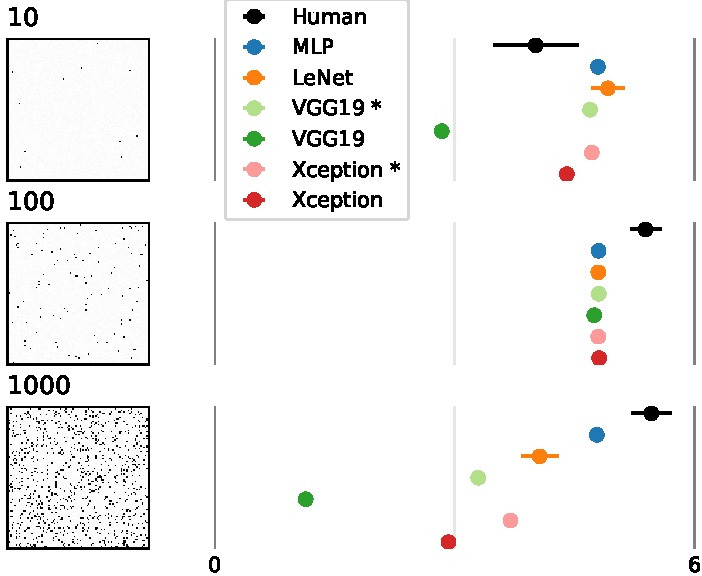
\includegraphics[width=0.9\linewidth]{weber_mlae_noise_all_NEW.pdf}
  \caption{\textbf{Computational results of the point cloud experiment.} \textit{Left:} We create 2D point clouds with 10, 100, and 1000 initial dots. Then, we add up to 10 new dots. For humans, it is possible to estimate how many dots are added if there are initially 10 points, but it is impossible to see how many dots are added when starting with 1000 dots. \textit{Right:} We let our networks regress the number of added dots and report MLAE and \change{bootstrapped} 95\% confidence intervals.}
	\label{fig:weber_law}
\end{figure}

\subsection{Results}

VGG is the only network able to solve the 10-dots version of the problem to within 10\% error, which itself is surprising. Most networks achieve close to midmean random performance, which is at $MLAE=4.8$. \change{Humans given a quick glance are better, solving the problem to within 17\% error or $MLAE=4.00$.} Moving to 100 dots, no network succeeds, and all networks achieve random performance. \change{For 100 and 1,000 dots, human performance is actually worse than random at 42\% and 44\% error respectively ($MLAE=5.39$ and $5.46$), as the participant response distributions skew towards estimating higher numbers of dots (we include response histograms in the supplemental material)}. At 1,000 dots, the larger-capacity networks perform better, which again is surprising, with VGG able to solve this problem to a low 3\% error. \change{This is explained by the fact that, with this many dots, the problem is easier solved as a summation problem rather than as a counting problem, which is a problem better suited to the multi-layer pooling architecture of CNNs.} As such, we only \textbf{partially reject 5.1}. 
%\JT{Unsatisfying!}

% Random performance was measured in MATLAB by:
% - Generating 1,000,000 random integers via uniform distribution to represent the random number of dots added.
% - Generating 1,000,000 random integers to represent the random guesses.
% - Computing the absolute error between these two vectors
% - Converting to MLAE
%
% In average error, random guesses should give 33% error
% But our human participants seem to be getting 42% error for 100, and 44% average error for 1,000.

%\JT{Relate to max pooling.} \JT{Why is 10 somewhat possible, but 100 is definitely not, but then 1,000 is possible again?}
